\chapter{Studiu de literatură}

\section{Prezentarea domeniului lucrării de diplomă}

\subsection{Introducere}

Revoluția modelelor bazate pe arhitectura transformer, apărută în 2017~\cite{vaswani2017attention} și a limbajelor lingvistice mari (Large Language Models - LLMs) a dus la o schimbare paradigmatică a abordării problemelor de procesare de limbaj natural. Modele precum BERT și GPT-3 au demonstrat capacități remarcabile în înțelegerea și generarea de text coerent, ceea ce a dus la o adoptare rapidă a LLM-urilor global, cercetarea despre LLM-uri devenind un punct central de interes. În Figura 1.1 se pot observa modelele SOTA de-a lungul anilor 2018-2024. Totuși, LLM-urile de sine stătătoare au o limitare fundamentală, cunoștințele lor sunt fixe, limitate la momentul antrenării, neputând fi actualizate fără a fi reantrenate~\cite{gao2024retrievalaugmentedgenerationlargelanguage}.     

\begin{figure}
    \centering
    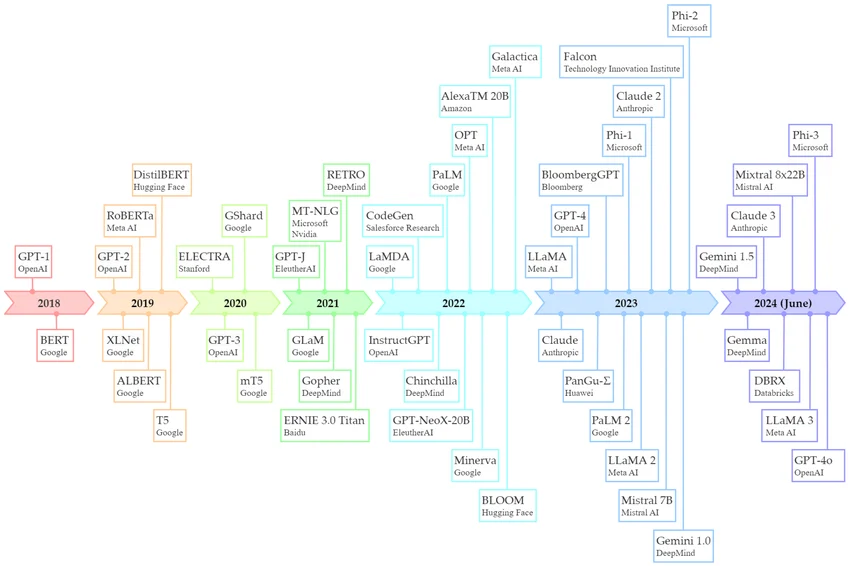
\includegraphics[width=1\linewidth]{Imagini/image.png}
    \caption{Evoluția modelelor lingvistice mari (LLMs) din 2018 până în 2024}
    \label{fig:placeholder}
\end{figure}

\subsection{Problema: Cunoștințe statice care duc la halucinații}

Fenomenul de „halucinație” reprezintă un răspuns aparent bine formulat, dar factual incorect, al unui LLM. Modelele generează text pe baza distribuției de probabilități a datelor cu care au fost antrenate, nu pe baza unor cunoștințe verificate. Pentru utilizatorul obișnuit, halucinațiile nu reprezintă un impediment major, însă există aplicații în care acestea sunt inacceptabile (medical, legal, financiar). 

În plus, informația încorporată în parametrii modelului este de natură „statică”, reflectă cunoștințele cunoscute la momentul antrenării. După antrenare, singura metodă de actualizare a informației este procesul costisitor de fine-tuning.

\subsection{Soluția: Retrieval-Augmented Generation}

Retrieval-Augmented Generation (RAG) este un tip de arhitectură de sistem de inteligență artificială care combină recuperarea informației relevante din surse externe cu capacitatea de generarea a LLM-urilor. În contextul unui sistem RAG, documentele relevante sunt recuperate dintr-o sursă externă de date, încorporate în contextul LLM-ului, iar în final, se generează un răspuns. Aceasta adresează ambele probleme simultan:

\begin{enumerate}
    \item Furnizează informația relevantă pentru un context factual corect, reducând astfel halucinațiile;
    \item Permite modificarea cunoștințelor și extensia contextului fără fine-tuning sau reantrenare.
\end{enumerate}

Termenul „RAG” a fost introdus în 2020 de către Patrick Lewis și colaboratorii săi de la Facebook AI Research (astăzi Meta AI) în lucrarea \textit{„Retrieval-Augmented Generation for Knowledge-Intensive NLP Tasks”}~\cite{lewis2020rag}.

\subsection{Formularea problemei: Extragerea relațiilor între entități}

Extragerea relațiilor între entități este o sarcină de bază în procesarea limbajului natural. Dat fiind un text, scopul este de a identifica entitățile menționate și relațiile dintre ele. De exemplu, din textul „Albert Einstein s-a născut în Ulm în 1879”, sistemul trebuie să extragă relațiile $(\text{Albert Einstein}, \text{născut în}, \text{Ulm})$ și $(\text{Albert Einstein}, \text{născut în an}, \text{1879})$.


Formal, fie $q$ o interogare și $\mathcal{D}=\{d_1,d_2,\dots,d_N\}$ o mulțime de documente. Un sistem RAG acționează în două etape. Prima etapă: un model de recuperare  $p_\eta(\cdot \mid q)$ alege o submulțime $\mathcal{Z} \subseteq \mathcal{D}$ de documente-candidat. A doua etapă: un model lingvistic mare generativ $p_\theta$ generează răspunsul $y$ condiționat de interogare dar și de documentele recuperate:
\begin{equation}
p(y \mid q) = \sum_{z \in \mathcal{Z}} p_\eta(z \mid q)\, p_\theta(y \mid q, z).
\label{eq:rag-marginal}
\end{equation}

RAG aduce o alternativă rețelelor neuronale de clasificare create pentru sarcini specifice. Sistemul recuperează pasaje relevante pentru fiecare pereche de entități, iar LLM-ul extrage relația pentru contextul recuperat, astfel generalizând pentru relații noi, fără reantrenare~\cite{gao2024retrievalaugmentedgenerationlargelanguage}.

\subsection{Relevanță și aplicații}

Sistemele RAG sunt relevante într-o gamă largă de domenii unde accesul dinamic la informații externe este esențial pentru generarea de răspunsuri de calitate~\cite{gao2024retrievalaugmentedgenerationlargelanguage}.
\begin{itemize}
    \item \textbf{Construirea grafurilor de cunoștințe}: Wikipedia, DBpedia, Freebase și alte baze de date semantice structurate sunt construite parțial prin extragerea automată a relațiilor
    \item \textbf{Asistenți inteligenți}: Chatbots și agenți de inteligență artificială care necesită cunoștințe actualizate constant
    \item \textbf{Domenii specializate}: Bioinformatică (extragerea relațiilor proteină-proteină), drept (identificarea precedenților), medicină (relații medicament-boală)
    \item \textbf{Indexare și căutare}: Motoarele de căutare moderne folosesc RAG pentru a livra răspunsuri directe
\end{itemize}

\section{Taxonomie}

\subsection{Motivația definirii unei taxonomii}

Domeniul RAG s-a dezvoltat rapid, producând numeroase variante și îmbunătățiri ale arhitecturii originale. Identificarea similarităților și diferențelor între abordări este dificilă fără o clasificare sistematică. Lucrările Gao et al. (2024) ~\cite{gao2024retrievalaugmentedgenerationlargelanguage} și Peng et al. (2025) ~\cite{peng2025graph} au fost folosite ca referință pentru această secțiune, care introduce o taxonomie bazată pe aspectele tehnologice cheie. Trebuie reținut că taxonomia este limitată la specificul acestei lucrări (RAG pentru extragerea relațiilor) și nu acoperă întreg domeniul.

\subsection{Criterii de clasificare}

\textbf{1. Tipul mecanismului de recuperare}

\begin{itemize}
    \item \textbf{Sparse retrieval}: Metode tradiționale de recuperare de IR (Information Retrieval) precum BM25, care se bazează pe potrivirea cuvintelor cheie. Rapid dar sensibil la variații lexicale și sinonime.
    \item \textbf{Dense retrieval}: Folosește reprezentări numerice a textului din documente (și interogarea către LLM) în spații vectoriale continue. Poate captura nuanțele semantice, dar costul computațional este mai ridicat.
    \item \textbf{Hybrid retrieval}: Combină sparse și dense prin fusion (ex. Reciprocal Rank Fusion), exploatând avantajele ambelor abordări. 
\end{itemize}

\textbf{2. Modul de integrare între recuperare și generare}

\begin{itemize}
    \item \textbf{Modular}: Componentele sunt decuplate. Recuperatorul și generatorul sunt independente și pot fi optimizate separat, oferind flexibilitate maximă.
    \item \textbf{End-to-end}: Recuperarea și generarea sunt cuplate, și sunt optimizate laolaltă, de regulă prin antrenare (gradient descent).
\end{itemize}

\textbf{3. Tipul sursei de cunoștințe}

\begin{itemize}
    \item \textbf{Nestructurată}: Documente text din diverse surse precum site-uri web (ex. articole Wikipedia), PDF-uri, documente Word. Pentru a putea fi procesate, necesită indexare și analiză semantică. 
    \item \textbf{Structurată}: Grafuri de cunoștințe cu entități și relații explicit modelate (DBpedia, Wikidata, Freebase), permitând navigare relațională.
    \item \textbf{Hibridă}: Combinație ale amândurora, exploatând avantaje complementare.
\end{itemize}

\textbf{4. Etapa augmentării}

\begin{itemize}
    \item \textbf{Pre-retrieval}: Optimizarea pre-recuperare prin extinderea și/sau reformularea interogării și descompunere semantică.
    \item \textbf{At-retrieval}: Optimizarea la momentul recuperării, prin selectarea parametrilor k, strategii adaptive de recuperare.
    \item \textbf{Post-retrieval}: Optimizare după recuperare, prin reranking, compactarea contextului și filtrare.
\end{itemize}

\subsection{Categorii principale}

\textbf{Naive RAG}

Paradigma originală din lucrarea Lewis et al. 2020~\cite{lewis2020rag}: indexare, urmată de recuperare de tip dense și generare. Recuperatorul și generatorul sunt elemente separate, și nu se folosesc optimizări. Este arhitectura de bază, folosită ca referință în majoritatea studiilor~\cite{lewis2020rag}, incluzând această teză. 

\textbf{Advanced RAG}

Adaugă optimizări pre- și post-recuperare, precum: rescriere a interogărilor, recuperare hibridă, și reranking cu model special antrenat. Dovedește îmbunătățiri semnificative, între 5 și 15\% pe benchmark-uri, cu costuri computaționale moderate. Lucrarea de față va implementa acest tip de arhitectură.

\textbf{Modular RAG}

Diferă de metodele Naive și Advanced în structură, fiecare element din arhitectura Modular RAG este un modul separat (ex. recuperare, memorare, rutare, predicție, căutare). Este cea mai adaptabilă/flexibilă arhitectură, însă introduce și cel mai înalt nivel de complexitate.

\textbf{Graph RAG}

Specifică pentru surse structurate de date: indexare pe grafuri de cunoștințe, recuperare utilizând relații semantice, generare pe bază de subgrafuri. Ideal pentru extragerea relațiilor din grafuri de cunoștințe dar necesită structurare prealabilă a datelor. Descris în detaliu de Peng et al. (2025)~\cite{peng2025graph}.

\section{Arhitectura generală a unui sistem de tip RAG}

Un sistem RAG funcționează în două faze: o fază offline de indexare și o fază online de inferență. Componentele principale sunt interogarea utilizatorului, baza de cunoștințe, mecanismul de recuperare și modelul generativ~\cite{gao2024retrievalaugmentedgenerationlargelanguage}.

\subsection{Componentele sistemului}

\textbf{Interogarea} reprezintă nevoia de informație a utilizatorului. În formele de bază, textul interogării este transmis direct mecanismului de recuperare. Sistemele avansate aplică mai întâi transformări ale interogării: reformulare semantică, extindere cu termeni sinonimi sau descompunere în sub-interogări, pentru a crește acoperirea și a reduce sensibilitatea față de formulări ambigue~\cite{gao2024retrievalaugmentedgenerationlargelanguage}.

\textbf{Baza de cunoștințe} este sursa externă din care se extrage informația. Documentele trec printr-o etapă de indexare offline: sunt împărțite în fragmente (eng. \textit{chunks}), codificate cu un model de reprezentare vectorială bazat pe arhitectura transformer~\cite{vaswani2017attention} și stocate într-o bază de date vectorială~\cite{karpukhin2020dpr}. Strategia de fragmentare influențează direct calitatea recuperării: fragmentele prea scurte pierd contextul necesar pentru identificarea relațiilor între entități, iar cele prea lungi diluează semnalul relevant.

\textbf{Mecanismul de recuperare} punctează fragmentele din baza vectorială în raport cu interogarea și returnează primele $k$ rezultate. Sistemele dense calculează similaritatea cosinus între vectorul interogării și vectorii fragmentelor~\cite{karpukhin2020dpr}. Sistemele sparse aplică potrivire ponderată de termeni, BM25 reprezentând standardul din domeniu~\cite{robertson2009bm25}. Sistemele hibride combină scorurile dense și sparse prin Reciprocal Rank Fusion (RRF)~\cite{cormack2009rrf}. Opțional, un model de reranking de tip cross-encoder poate rafina ordinea inițială a fragmentelor recuperate.

\textbf{Modelul generativ} primește contextul augmentat, format din interogarea originală și fragmentele recuperate, și produce răspunsul final~\cite{lewis2020rag}. Arhitecturile orientate spre fidelitate constrâng explicit modelul să fundamenteze răspunsurile pe dovezile recuperate, reducând astfel rata de halucinații~\cite{asai2023self}.

\subsection{Fluxul de date}

Figura~\ref{fig:rag-arch} ilustrează cele două trasee ale fluxului de date. Offline, documentele sunt procesate o singură dată: fragmentate, codificate și stocate în baza vectorială. Online, fiecare interogare parcurge procesarea interogării, recuperarea fragmentelor, augmentarea contextului și generarea răspunsului.

\begin{figure}[htbp]
    \centering
    \begin{tikzpicture}[
        node distance=1.0cm and 1.4cm,
        proc/.style={rectangle, rounded corners, draw=black!70, fill=blue!8, thick, align=center, minimum width=2.1cm, minimum height=0.85cm, font=\small},
        store/.style={cylinder, shape border rotate=90, aspect=0.25, draw=black!70, fill=green!12, thick, align=center, minimum width=2.1cm, font=\small},
        arr/.style={-{Stealth[length=2.5mm]}, thick}
    ]
    \node[proc] (docs) {Documente};
    \node[proc, right=of docs] (chunk) {Fragmentare};
    \node[proc, right=of chunk] (emb) {Codificare\\vectorială};
    \node[store, right=of emb] (vdb) {Bază de\\date vectorială};
    \draw[arr] (docs) -- (chunk);
    \draw[arr] (chunk) -- (emb);
    \draw[arr] (emb) -- (vdb);
    \node[proc, below=2.0cm of docs] (query) {Interogare};
    \node[proc, right=of query] (qproc) {Procesare\\interogare};
    \node[proc, right=of qproc] (retr) {Recuperare\\+ Reranking};
    \node[proc, right=of retr] (gen) {Model\\generativ};
    \node[proc, right=of gen] (out) {Răspuns};
    \draw[arr] (query) -- (qproc);
    \draw[arr] (qproc) -- (retr);
    \draw[arr] (retr) -- (gen);
    \draw[arr] (gen) -- (out);
    \draw[arr] (vdb) |- (retr);
    \end{tikzpicture}
    \caption{Arhitectura generală a unui sistem RAG: indexare offline (sus) și inferență online (jos)~\cite{gao2024retrievalaugmentedgenerationlargelanguage, karpukhin2020dpr}.}
    \label{fig:rag-arch}
\end{figure}

\section{Metode și modele RAG}

\subsection{Naive RAG}

Formularea originală a RAG, propusă de Lewis et al. (2020)~\cite{lewis2020rag}, combină un recuperator bazat pe Dense Passage Retrieval (DPR) cu un model generativ de tip sequence-to-sequence, optimizate parțial în comun. Fluxul de lucru este liniar: indexare, recuperare densă, generare. Această variantă servește ca referință în majoritatea studiilor din literatura de specialitate~\cite{gao2024retrievalaugmentedgenerationlargelanguage}.

Limitările Naive RAG sunt bine documentate: sistemul nu gestionează variațiile lexicale (sinonime, parafrazări), nu evaluează calitatea documentelor recuperate și nu filtrează fragmentele irelevante înainte de generare~\cite{gao2024retrievalaugmentedgenerationlargelanguage}. Cu toate acestea, simplitatea sa face din Naive RAG un punct de plecare util pentru orice evaluare comparativă, inclusiv în cadrul acestei teze.

\subsection{Advanced RAG}

Advanced RAG adaugă optimizări pre-recuperare și post-recuperare față de varianta de bază~\cite{gao2024retrievalaugmentedgenerationlargelanguage}. Pre-recuperare: fragmentare semantică, îmbogățirea fragmentelor cu metadate, generare de interogări multiple. Post-recuperare: reranking cu model cross-encoder, compactarea contextului pentru a reduce zgomotul din prompt. Scorurile dense și sparse sunt combinate prin RRF~\cite{cormack2009rrf}. Studiile raportează îmbunătățiri de 5--15\% față de Naive RAG pe benchmark-uri standard.

Pentru extragerea relațiilor, optimizările post-recuperare sunt relevante în mod direct: identificarea corectă a unei relații necesită fragmente care conțin simultan ambele mențiuni de entitate și indiciile lexicali ai relației. Reranking-ul crește șansa ca aceste fragmente să ajungă în contextul modelului generativ. Aceasta este arhitectura pe care lucrarea de față o implementează și evaluează în partea experimentală.

\subsection{Hypothetical Document Embeddings (HyDE)}

HyDE~\cite{gao2023hyde} folosește un model de limbaj pentru a genera un pseudo-document care ar conține răspunsul la interogare. Acest pseudo-document este codificat și se caută documente reale similare prin recuperare densă. Encoderele contrastive eliminată erorile factuale din pseudo-document, păstrând tiparele de relevanță semantică~\cite{gao2023hyde}.

Avantajul principal al HyDE este că îmbunătățește recuperarea fără a necesita date de antrenare etichetate pentru interogări. Dezavantajul este dependența de calitatea generării inițiale: un pseudo-document slab generat poate conduce recuperarea în direcția greșită.

\subsection{REALM, Fusion-in-Decoder și RETRO}

REALM~\cite{guu2020realm} integrează recuperarea chiar în etapa de pre-antrenare, tratând recuperatorul ca o variabilă latentă optimizată împreună cu modelul de limbaj. Abordarea arată că un recuperator co-antrenat cu generatorul înțelege mai bine ce tipuri de documente sunt utile pentru diferite sarcini.

Fusion-in-Decoder (FiD)~\cite{izacard2021fid} codifică fiecare pasaj recuperat independent prin encoder, dar realizează fuziunea la nivelul decoderului. Astfel, modelul poate agrega dovezi din surse multiple fără a sufoca encoderele cu un context prea lung. RETRO~\cite{borgeaud2022retro} extinde această idee la scara corpusurilor de zeci de trilioane de tokenuri, fără a crește proporțional numărul de parametri ai modelului, obținând eficiență parametrică pe seama unei infrastructuri mai complexe.

\subsection{RAPTOR}

RAPTOR~\cite{sarthi2024raptor} construiește un arbore de rezumate de jos în sus: fragmentele de text sunt grupate în clustere, rezumate, iar procesul se repetă recursiv, generând niveluri de abstractizare din ce în ce mai înalte. La inferență, recuperarea operează pe acest arbore și poate agrega informații de la mai multe niveluri de abstractizare simultan.

Metoda obține rezultate bune pe sarcini care necesită raționament distribuit pe mai multe documente~\cite{sarthi2024raptor}. Avantajul față de recuperarea standard este că furnizează modelului generativ atât detalii de granularitate fină, cât și context global. Dezavantajul constă în costul de construire și actualizare a arborelui.

\subsection{Corrective RAG (CRAG)}

CRAG~\cite{yan2024crag} adaugă un evaluator al calității documentelor recuperate. Când relevanța fragmentelor este insuficientă, sistemul declanșează acțiuni corective: recuperare suplimentară sau căutare pe web, urmată de rafinarea cunoștințelor prin descompunere și recompunere a informației. Dacă documentele recuperate sunt de bună calitate, fluxul rămâne cel standard.

Mecanismul de auto-corecție face sistemul mai robust față de recuperările greșite și reduce riscul extragerii unei relații dintr-un context irelevant. CRAG este una dintre primele abordări care tratează explicit eșecul recuperării ca un caz de gestionat, nu ca o excepție rară.

\subsection{Self-RAG}

Self-RAG~\cite{asai2023self} antrenează un singur model să decidă adaptiv când să recupereze, când să genereze și când să critice propriile răspunsuri, folosind tokenuri speciale de reflecție introduse în vocabularul modelului. Modelul evaluează relevanța fragmentului recuperat și gradul de fundamentare factuală a răspunsului generat înainte de a-l returna utilizatorului.

Față de CRAG, care utilizează un evaluator extern, Self-RAG internalizează întregul proces de evaluare și corecție. Fidelitatea și controlabilitatea cresc~\cite{asai2023self}. Pentru extragerea relațiilor, posibilitatea de a verifica dacă tipul de relație prezis este susținut de dovezile recuperate este utilă în mod direct, deoarece reduce numărul de relații extrase din fragmente slab relevante.

\subsection{Adaptive-RAG și FLARE}

Adaptive-RAG~\cite{jeong2024adaptiverag} alege dinamic strategia de recuperare potrivită pentru fiecare interogare, fără recuperare, cu recuperare unică sau cu recuperare iterativă, pe baza complexității estimate cu un clasificator mic antrenat separat. Interogările simple nu necesită recuperare; cele complexe, care implică mai mulți pași de raționament, beneficiază de recuperare iterativă.

FLARE~\cite{jiang2023flare} abordează problema diferit, prin recuperare activă: modelul generează propoziția următoare și, atunci când detectează tokenuri cu probabilitate scăzută (indiciu de incertitudine), folosește predicția respectivă ca interogare și recuperează documente suplimentare înainte de a regenera propoziția. Recuperarea iterativă din Adaptive-RAG ajută la identificarea relațiilor distribuite pe mai multe documente, iar FLARE reduce halucinațiile în extragerea pe texte lungi.

\subsection{GraphRAG și HippoRAG}

GraphRAG~\cite{edge2024graphrag} construiește un graf de cunoștințe din corpus prin extragerea entităților și relațiilor, structurând informația în comunități ierarhice rezumate. Recuperarea operează pe acest graf prin traversarea relațiilor semantice, permițând raționamentul global, nu doar căutarea locală de fragmente similare.

HippoRAG~\cite{gutierrez2024hipporag} integrează un model de limbaj, un graf de cunoștințe și Personalised PageRank: corpusul este transformat într-un graf fără schemă predefinită, iar conceptele din interogare servesc ca noduri de pornire pentru propagarea pe graf. Ambele abordări se înscriu în direcția de cercetare Graph RAG descrisă de Peng et al. (2025)~\cite{peng2025graph}. Avantajul comun este descoperirea relațiilor implicite distribuite în mai multe pasaje, ceea ce le face relevante în mod direct pentru sarcina de extragere a relațiilor. Limitarea comună este costul de construire și actualizare a grafului.

\subsection{RAG pentru contexte lungi și aplicații specializate}

Creșterea numărului de pasaje recuperate nu garantează îmbunătățirea performanței. Pasajele irelevante din contexte lungi degradează calitatea generării, un fenomen documentat de Jin et al. (2024)~\cite{jin2024long}. Problema selectivității devine la fel de importantă ca problema acoperirii.

Alte extensii documentate în literatura recentă includ RAG multimodal, care integrează documente text, imagini, audio și video~\cite{mei2025survey}, MMed-RAG pentru modele vizuale din domeniul medical~\cite{xia2024mmed}, RAP pentru personalizarea răspunsurilor în funcție de preferințele utilizatorului~\cite{hao2025rap} și abordări de recuperare din colecții de mii de documente~\cite{chen2025document}.

\section{Metrici de evaluare}

Evaluarea unui sistem RAG este mai complexă decât evaluarea unui model generativ izolat, deoarece performanța globală depinde atât de componenta de recuperare, cât și de cea de generare~\cite{gao2024retrievalaugmentedgenerationlargelanguage}. O recuperare slabă limitează calitatea răspunsului indiferent de capacitățile modelului generativ.

\subsection{Metrici de recuperare}

\textbf{Precizia la rang $k$} (Precision@$k$) este proporția documentelor relevante printre primele $k$ rezultate recuperate:
\begin{equation}
\text{Precision@}k = \frac{|\{\text{relevante}\} \cap \{\text{top-}k\}|}{k}.
\label{eq:precision}
\end{equation}

\textbf{Recuperarea la rang $k$} (Recall@$k$) reprezintă proporția tuturor documentelor relevante care au fost efectiv recuperate:
\begin{equation}
\text{Recall@}k = \frac{|\{\text{relevante}\} \cap \{\text{top-}k\}|}{|\{\text{relevante}\}|}.
\label{eq:recall}
\end{equation}

\textbf{Mean Reciprocal Rank} (MRR) măsoară rangul primului document relevant, mediat peste $|Q|$ interogări:
\begin{equation}
\text{MRR} = \frac{1}{|Q|} \sum_{i=1}^{|Q|} \frac{1}{\text{rang}_i}.
\label{eq:mrr}
\end{equation}

Aceste metrici sunt calculate față de un set de documente relevante adnotate manual. În practică, Recall@$k$ este adesea mai informativă decât Precision@$k$ pentru sistemele RAG, deoarece un document relevant ratat nu poate fi recuperat ulterior de modelul generativ~\cite{karpukhin2020dpr}.

\subsection{Metrici de generare}

\textbf{Exact Match} (EM) este o metrică binară care indică potrivirea completă, token cu token, față de răspunsul de referință. Este strictă și potrivită pentru răspunsuri scurte sau factuale.

\textbf{Scorul $F_1$} la nivel de token echilibrează precizia $P$ și recuperarea $R$ față de răspunsul de referință:
\begin{equation}
F_1 = \frac{2 \cdot P \cdot R}{P + R}.
\label{eq:f1}
\end{equation}

Pentru răspunsuri mai lungi, unde potrivirea exactă este irealistă, se utilizează suprapunerea de $n$-grame calculată cu metricile ROUGE și BLEU~\cite{gao2024retrievalaugmentedgenerationlargelanguage}. ROUGE-L măsoară cel mai lung subșir comun, captând ordinea parțială a tokenurilor.

\subsection{Metrici specifice sistemelor RAG}

Metricile clasice de generare nu surprind fenomenul halucinației în contextul RAG, deoarece nu verifică dacă răspunsul este fundamentat pe contextul recuperat. Cadrul RAGAS~\cite{es2024ragas} introduce metrici dedicate:

\textbf{Fidelitatea} (faithfulness) măsoară proporția afirmațiilor din răspuns care pot fi deduse din contextul recuperat. O fidelitate de 1.0 indică un răspuns complet susținut de dovezile furnizate.

\textbf{Relevanța răspunsului} (answer relevancy) măsoară în ce grad răspunsul adresează interogarea originală, penalizând răspunsurile complete factual, dar tangențiale față de întrebare.

\textbf{Precizia contextului} și \textbf{recuperarea contextului} evaluează calitatea recuperării din perspectiva generării: câte dintre fragmentele recuperate sunt cu adevărat necesare și câte dintre fragmentele necesare au fost recuperate~\cite{es2024ragas}. Aceste metrici sunt centrale pentru sistemele orientate spre fidelitate~\cite{asai2023self} și constituie principalele criterii de comparare în demonstratorul din această teză.

\subsection{Dificultăți în evaluarea extragerii relațiilor}

Evaluarea extragerii relațiilor se realizează cu scorurile micro și macro $F_1$ calculate pe tipurile de relații. Micro-$F_1$ ponderează fiecare instanță egal, favorizând tipurile de relații frecvente. Macro-$F_1$ tratează fiecare tip de relație egal, indiferent de frecvența sa.

Există două dificultăți structurale. Prima este distribuția dezechilibrată a tipurilor de relații în seturile de date existente, care face ca micro-$F_1$ să fie adesea înșelătoare~\cite{tan2022redocred}. A doua este problema falselor negative: relații corecte neanotate în setul de referință duc la subestimarea performanței reale. Re-DocRED~\cite{tan2022redocred} a demonstrat că DocRED~\cite{yao2019docred} conținea un număr semnificativ de astfel de false negative.

Metricile de fidelitate nu reflectă direct corectitudinea tipului de relație extras: un sistem poate fi fidel față de contextul recuperat, dar contextul însuși poate conține relații ambigue sau greșit formulate. Prin urmare, evaluarea completă a unui sistem RAG pentru extragerea relațiilor necesită atât metrici de fidelitate, cât și metrici specifice extragerii.

\section{Baze de date}

\subsection{Seturi de date pentru sisteme RAG}

\textbf{SQuAD}~\cite{rajpurkar-etal-2016-squad} (Stanford Question Answering Dataset) leagă întrebări de pasaje din Wikipedia, răspunsul reprezentând un fragment de text contiguu extras din pasaj. Setul conține 100.000 de întrebări construite de adnotatori umani, ceea ce îl face un standard pentru evaluarea recuperării și extracției.

\textbf{Natural Questions}~\cite{kwiatkowski2019nq} conține întrebări reale adresate motorului de căutare Google, perechi cu pagini Wikipedia. Spre deosebire de SQuAD, întrebările nu sunt construite cu pasajele în față, ceea ce le face mai reprezentative pentru scenariile reale de utilizare. Setul de date include atât răspunsuri scurte, cât și lungi.

\textbf{TriviaQA}~\cite{joshi2017triviaqa} este un set de perechi întrebare-răspuns colectate din resurse trivia, însoțite de documente justificative găsite independent prin căutare web. Dificultatea suplimentară față de SQuAD este că documentele justificative nu sunt garantat să conțină răspunsul.

\textbf{HotpotQA}~\cite{yang2018hotpotqa} este un benchmark care necesită raționament pe mai multe documente simultan. Fiecare întrebare este adnotată cu faptele justificative din mai multe articole Wikipedia, forțând sistemele să realizeze recuperare și raționament multi-hop. Este relevant pentru extragerea relațiilor care implică mai multe entități intermediare.

\textbf{CRAG}~\cite{yang2024cragbench} (Comprehensive RAG Benchmark) conține 4.409 perechi QA generate cu API-uri de căutare web și de grafuri de cunoștințe. Acoperă cinci domenii și opt categorii de întrebări cu niveluri variabile de dinamism temporal, ceea ce îl face util pentru evaluarea robustetei față de informații care se schimbă în timp.

\subsection{Seturi de date pentru extragerea relațiilor}

\textbf{T-REx}~\cite{elsahar2018trex} este un set de aliniament la scară largă între rezumatele Wikipedia și tripletele Wikidata: 11 milioane de triplete aliniate cu 3,09 milioane de rezumate. Structura sa face T-REx potrivit pentru evaluarea sistemelor care combină recuperarea din text liber cu validarea față de grafuri de cunoștințe. Reprezintă setul de date utilizat în partea experimentală a acestei teze.

\textbf{WebNLG}~\cite{gardent2017webnlg} furnizează perechi date-text pornind de la triplete RDF din DBpedia. Setul de date are aplicații atât în extragerea relațiilor, cât și în verbalizarea datelor structurate, deoarece fiecare triplet este însoțit de fraze naturale care îl exprimă.

\textbf{SemEval-2010 Task 8}~\cite{hendrickx2010semeval} este un benchmark de clasificare a relațiilor semantice între perechi nominale la nivel de propoziție, cu nouă tipuri de relații direcționale plus o clasă negativă. Este utilizat frecvent ca referință pentru compararea metodelor de extragere a relațiilor la nivel de propoziție.

\textbf{TACRED}~\cite{zhang2017tacred} este un set de date de mari dimensiuni construit din articole de știri și rapoarte ale agenției Associated Press, cu 41 de tipuri de relații și o clasă negativă predominantă. Dezechilibrul accentuat între clase face evaluarea macro-$F_1$ mai informativă decât micro-$F_1$.

\textbf{DocRED}~\cite{yao2019docred} extinde extragerea relațiilor la nivel de document, necesitând raționament inter-propoziții. Un număr semnificativ de relații implică entități menționate în propoziții diferite, ceea ce face DocRED mai dificil decât seturile sentence-level.

\textbf{Re-DocRED}~\cite{tan2022redocred} corectează problema falselor negative din DocRED prin reannotare manuală sistematică. Studiul original a arătat că o parte considerabilă din relațiile corecte din DocRED nu fuseseră adnotate, ceea ce subestima performanța modelelor evaluate pe setul original.

\begin{table}[htbp]
\centering
\small
\begin{tabularx}{\textwidth}{l l c X}
\toprule
\textbf{Set de date} & \textbf{Sarcină} & \textbf{Nivel} & \textbf{Caracteristici principale} \\
\midrule
SQuAD & QA extractiv & Propoziție & Fragment de text ca răspuns \\
Natural Questions & QA & Document & Întrebări reale, răspuns scurt/lung \\
HotpotQA & QA multi-hop & Multi-document & Fapte justificative adnotate \\
CRAG & QA factual & Web / GC & 4.409 perechi, dinamism temporal \\
T-REx & Extragere relații & Document & Aliniament text-triplete Wikidata \\
WebNLG & Extragere/verbalizare & Triplete RDF & Perechi date-text \\
SemEval-2010 T8 & Extragere relații & Propoziție & Relații nominale, 9 tipuri \\
TACRED & Extragere relații & Propoziție & 41 tipuri de relații \\
DocRED & Extragere relații & Document & Raționament inter-propoziții \\
Re-DocRED & Extragere relații & Document & Corectare false negative \\
\bottomrule
\end{tabularx}
\caption{Comparație a seturilor de date pentru evaluarea RAG și extragerea relațiilor~\cite{rajpurkar-etal-2016-squad, kwiatkowski2019nq, yang2018hotpotqa, yang2024cragbench, elsahar2018trex, gardent2017webnlg, hendrickx2010semeval, zhang2017tacred, yao2019docred, tan2022redocred}.}
\label{tab:datasets}
\end{table}

\section{Limitări și provocări}

\textbf{Calitatea recuperării.} Documentele irelevante sau parțial relevante induc în eroare modelul generativ, ducând la halucinații chiar și atunci când există o sursă externă de informație~\cite{gao2024retrievalaugmentedgenerationlargelanguage, yan2024crag}. Recuperarea fixă, neadaptivă, nu poate evalua sau corecta automat rezultatele slabe~\cite{asai2023self}. Fragmentele care conțin una dintre entitățile căutate, dar nu și relația relevantă, sunt o sursă frecventă de erori în extragerea relațiilor.

\textbf{Integrarea contextelor lungi.} Creșterea numărului de pasaje recuperate nu îmbunătățește neapărat performanța. Pasajele irelevante din contexte lungi degradează calitatea textului generat~\cite{jin2024long}. Fenomenul, denumit uneori \textit{lost in the middle}, arată că modelele generative tind să ignore informațiile aflate la mijlocul unui context lung, chiar dacă acestea sunt relevante.

\textbf{Limitări ale datelor și metricilor.} Seturile de date pentru extragerea relațiilor au distribuții dezechilibrate și conțin false negative~\cite{tan2022redocred}. Metricile de fidelitate nu reflectă direct corectitudinea tipului de relație extras~\cite{es2024ragas}. Construirea de seturi de date de calitate la nivel de document este costisitoare și lentă.

\textbf{Dificultăți în extragerea relațiilor.} Identificarea unei relații necesită adesea agregarea dovezilor din mai multe propoziții sau documente, ceea ce presupune un raționament inter-propoziție dificil de realizat într-un singur pas de recuperare~\cite{yao2019docred, edge2024graphrag}. Relațiile implicite, care nu apar formulat explicit în text, reprezintă o provocare suplimentară.

\textbf{Costul computațional.} Indexarea densă, recuperarea hibridă, rerankingul cu cross-encoder și generarea cu LLM-uri sunt toate operații care consumă resurse semnificative~\cite{karpukhin2020dpr, borgeaud2022retro}. Abordările adaptive și active implică recuperare iterativă, cu mai multe apeluri la model pe interogare~\cite{jiang2023flare, jeong2024adaptiverag}. Metodele bazate pe grafuri adaugă costul construirii și actualizării grafului de cunoștințe~\cite{sarthi2024raptor, gutierrez2024hipporag}. În absența unor resurse computaționale ample, aceste cerințe limitează scala la care sistemele pot fi evaluate sau folosite în producție.

\section{Concluzii}

Capitolul de față a prezentat contextul teoretic al sistemelor RAG aplicate extragerii relațiilor între entități. Au fost discutate limitările cunoștințelor parametrice ale modelelor lingvistice mari~\cite{gao2024retrievalaugmentedgenerationlargelanguage, lewis2020rag} și motivul pentru care augmentarea cu recuperare externă reprezintă o soluție practică, urmată de o taxonomie specifică acestei teze, construită pe criteriile tipului de mecanism de recuperare, al modului de integrare recuperare-generare și al sursei de cunoștințe.

Analiza literaturii arată că robustețea sistemelor RAG depinde în primul rând de calitatea recuperării și de capacitatea de a evalua adaptiv dovezile recuperate~\cite{asai2023self, yan2024crag}. Extragerea relațiilor beneficiază cel mai mult de structurile de grafuri de cunoștințe și de abordările cu raționament la nivel de document~\cite{edge2024graphrag, gutierrez2024hipporag, yao2019docred}. Provocările deschise rămân integrarea contextelor lungi~\cite{jin2024long}, limitările metricilor și datelor~\cite{tan2022redocred, es2024ragas} și costul computațional~\cite{borgeaud2022retro}.

Lucrarea se plasează la intersecția optimizării recuperării cu dezvoltarea de mecanisme generative care integrează explicit dovezile recuperate. Demonstratorul propus compară Naive RAG cu Advanced RAG, pornind de la observația că optimizările pre- și post-recuperare conduc la îmbunătățiri măsurabile ale fidelității și relevanței răspunsurilor~\cite{gao2024retrievalaugmentedgenerationlargelanguage, es2024ragas}, aspecte cu impact direct asupra corectitudinii relațiilor extrase.